% =============================================================================
% NANOPB PROTOCOL SPECIFICATION
% =============================================================================

\section{Nanopb (Protobuf) Protocol with ARQ and CRC for SPI Communication}

\subsection{Executive Summary}

\textbf{Overview:} Protocol Buffers (nanopb) encapsulated in frames with CRC-32 and Automatic Repeat Request (ARQ) for reliable SPI communication between RPi5 and ESP32-S3.

\noindent\makebox[\textwidth]{%
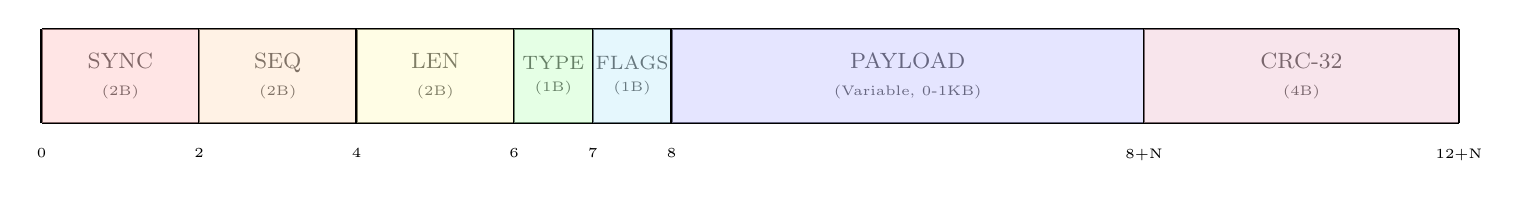
\begin{tikzpicture}[
    font=\small,
    offset/.style={font=\tiny, anchor=north}
]
    % Main frame bar - proportional widths (1 byte = 1 unit for fixed fields)
    \draw[thick] (0,0) -- (18,0);
    \draw[thick] (0,1.2) -- (18,1.2);

    % SYNC (2 bytes = 2 units)
    \draw[thick] (0,0) -- (0,1.2);
    \node[font=\footnotesize, align=center] at (1, 0.6) {SYNC\\{\tiny (2B)}};
    \fill[red!20, opacity=0.5] (0,0) rectangle (2,1.2);

    % SEQ (2 bytes = 2 units)
    \draw[thick] (2,0) -- (2,1.2);
    \node[font=\footnotesize, align=center] at (3, 0.6) {SEQ\\{\tiny (2B)}};
    \fill[orange!20, opacity=0.5] (2,0) rectangle (4,1.2);

    % LEN (2 bytes = 2 units)
    \draw[thick] (4,0) -- (4,1.2);
    \node[font=\footnotesize, align=center] at (5, 0.6) {LEN\\{\tiny (2B)}};
    \fill[yellow!20, opacity=0.5] (4,0) rectangle (6,1.2);

    % TYPE (1 byte = 1 unit)
    \draw[thick] (6,0) -- (6,1.2);
    \node[font=\scriptsize, align=center] at (6.5, 0.6) {TYPE\\{\tiny (1B)}};
    \fill[green!20, opacity=0.5] (6,0) rectangle (7,1.2);

    % FLAGS (1 byte = 1 unit)
    \draw[thick] (7,0) -- (7,1.2);
    \node[font=\scriptsize, align=center] at (7.5, 0.6) {FLAGS\\{\tiny (1B)}};
    \fill[cyan!20, opacity=0.5] (7,0) rectangle (8,1.2);

    % PAYLOAD (variable, 6 units to show it's typically the largest field)
    \draw[thick] (8,0) -- (8,1.2);
    \node[font=\footnotesize, align=center] at (11, 0.6) {PAYLOAD\\{\tiny (Variable, 0-1KB)}};
    \fill[blue!20, opacity=0.5] (8,0) rectangle (14,1.2);

    % CRC-32 (4 bytes = 4 units)
    \draw[thick] (14,0) -- (14,1.2);
    \node[font=\footnotesize, align=center] at (16, 0.6) {CRC-32\\{\tiny (4B)}};
    \fill[purple!20, opacity=0.5] (14,0) rectangle (18,1.2);

    \draw[thick] (18,0) -- (18,1.2);

    % Byte offset labels
    \node[offset] at (0,-0.2) {0};
    \node[offset] at (2,-0.2) {2};
    \node[offset] at (4,-0.2) {4};
    \node[offset] at (6,-0.2) {6};
    \node[offset] at (7,-0.2) {7};
    \node[offset] at (8,-0.2) {8};
    \node[offset] at (14,-0.2) {8+N};
    \node[offset] at (18,-0.2) {12+N};
\end{tikzpicture}%
}

\textbf{System Constraints:}
\begin{itemize}
    \item ESP32-S3-WROOM-1-N16: 16MB flash, 512KB SRAM, NO PSRAM
    \item 100Hz SPI communication (10ms period)
    \item 250Hz motor control loop (4ms period)
    \item Static allocation only (no malloc)
\end{itemize}

\subsubsection{Control Loop Frequency Rationale}

\textbf{Why different loop rates?}

The nested loop architecture follows classic control systems design. The outer loop (SPI at 100Hz) handles command distribution and telemetry collection, while the inner loop (PID at 250Hz) responds quickly to motor dynamics. Running PID at 2.5 times the communication rate ensures smooth control between commands without wasting CPU on excessive computation.

\textbf{Why 250Hz for motor control?}

This is a Nyquist sampling consideration. With DC gearmotors at 210 RPM (3.5 Hz mechanical speed) and a first-order time constant $\tau = 75$ ms (cutoff frequency $f_c = 1/(2\pi \tau) \approx 2.1$ Hz), the 250Hz control rate provides approximately 60 times oversampling of the mechanical dynamics - well above the 2 times Nyquist minimum.

While the ESP32 could easily run the PID loop at 1kHz or higher, doing so would not improve control quality because the motor mechanics are the limiting factor, not the computational speed. The physical system cannot respond faster than its time constant allows. Running at 250Hz balances:

\begin{itemize}
    \item Adequate sampling of motor dynamics (60 times oversampling)
    \item Efficient CPU utilization (4 motors $\times$ PID + encoder reads)
    \item Low latency between velocity commands and motor response
    \item Power efficiency (fewer ADC conversions, GPIO reads, and computations)
\end{itemize}

For context, control loop frequencies should match system dynamics:
\begin{itemize}
    \item DC gearmotors: 50-500 Hz typical
    \item High-speed servos: 1-10 kHz
    \item Motor current control: 10-50 kHz
    \item Temperature control: 0.1-10 Hz
\end{itemize}

\subsection{Key Design Decisions}

\subsubsection{Protocol Stack}
\label{sec:protocol-stack}

\noindent\makebox[\textwidth]{%
\begin{tikzpicture}[
    font=\small,
    node distance = 0cm,
    layer/.style={
        draw,
        thick,
        rectangle,
        minimum width=15cm,
        minimum height=1.3cm,
        align=left,
        text width=14.5cm
    },
]
    \node[layer, fill=red!20] (app) at (0,0) {\textbf{Application} \hfill Motor Commands, Telemetry, OTA Updates};
    \node[layer, fill=orange!20, below=of app] (serial) {\textbf{Serialization} \hfill nanopb (Protocol Buffers) with static allocation};
    \node[layer, fill=yellow!20, below=of serial] (arq) {\textbf{ARQ} \hfill Stop-and-Wait (SEQ/ACK/NACK, 8ms timeout)};
    \node[layer, fill=green!20, below=of arq] (frame) {\textbf{Frame} \hfill SYNC (2B) + Header (6B) + Payload + CRC-32 (4B)};
    \node[layer, fill=blue!20, below=of frame] (transport) {\textbf{Transport} \hfill SPI peripheral mode with DMA (10 Mbps)};
    \draw[->, very thick, gray] (-8, 1) -- (-8, -6) node[midway, left, rotate=90, xshift=-0.5cm, yshift=0.5cm] {Data Flow};
\end{tikzpicture}%
}

\subsubsection{Byte Order and Standards Compliance}

The protocol follows established standards for byte ordering to ensure cross-platform compatibility:

\begin{table}[H]
\centering
\caption{Byte Order Standards by Protocol Field}
\label{tab:byte-order-standards}
\begin{tabular}{|l|l|l|l|}
\hline
\textbf{Field} & \textbf{Byte Order} & \textbf{Standard} & \textbf{Rationale} \\
\hline
SYNC & Big-endian & RFC 1700 & Network byte order for headers \\
SEQ & Big-endian & RFC 1700 & Network byte order for headers \\
LEN & Big-endian & RFC 1700 & Network byte order for headers \\
TYPE & N/A (1 byte) & -- & Single byte, no endianness \\
FLAGS & N/A (1 byte) & -- & Single byte, no endianness \\
CRC-32 & Little-endian & IEEE 802.3 & Standard CRC-32 polynomial \\
\hline
\end{tabular}
\end{table}

\textbf{SYNC Magic Word (0x55AA):} The frame synchronization marker uses the distinctive bit pattern 0x55AA (binary: 0101010101010101 in big-endian wire format). This alternating pattern is easily recognizable and unlikely to appear in random data, making it ideal for frame alignment. The value 0x55AA is transmitted as bytes \texttt{[0x55, 0xAA]} on the wire.

\textbf{RFC 1700 (Network Byte Order):} All multi-byte header fields (SYNC, SEQ, LEN) use big-endian format following RFC 1700 ``Assigned Numbers'' standard. This ensures compatibility when communicating between different architectures (ARM RPi5 and Xtensa ESP32, both little-endian internally).

\textbf{IEEE 802.3 (CRC-32):} The frame checksum uses IEEE 802.3 polynomial (0x04C11DB7) in little-endian format, matching the ESP32 ROM CRC implementation and standard Ethernet CRC libraries. This allows zero-copy CRC validation using hardware accelerators where available.

\vspace{0.2cm}

\noindent\colorbox{keyinsightcolor}{\parbox{\dimexpr\linewidth-2\fboxsep}{%
\textbf{Key Insight:} Mixed byte orders are intentional — headers follow network standards for cross-platform compatibility, while CRC follows IEEE 802.3 for hardware acceleration and library compatibility.
}}

\vspace{0.3cm}

\subsubsection{Memory Budget}

\begin{table}[H]
    \centering
    \begin{minipage}{0.47\textwidth}
        \centering
        \small
        \caption{SRAM Usage (512 KB total)}
        \label{tab:sram-usage}
        {\setlength{\tabcolsep}{3pt}
        \begin{tabular}{lrr}
            \toprule
            \textbf{Component} & \textbf{Size (KB)} & \textbf{Usage (\%)} \\
            \midrule
            DMA double-buffer & 8.0 & 1.56 \\
            RX/TX buffers & 2.0 & 0.39 \\
            Protobuf structs & 1.5 & 0.29 \\
            ARQ state & 4.0 & 0.78 \\
            \midrule
            \textbf{Total} & \textbf{15.5} & \textbf{3.03} \\
            \bottomrule
        \end{tabular}}
    \end{minipage}\hfill%
    \begin{minipage}{0.47\textwidth}
        \centering
        \small
        \caption{Flash Usage (16 MB total)}
        \label{tab:flash-usage}
        {\setlength{\tabcolsep}{3pt}
        \begin{tabular}{lrr}
            \toprule
            \textbf{Component} & \textbf{Size (KB)} & \textbf{Usage (\%)} \\
            \midrule
            Generated protobuf & 80 & 0.49 \\
            Nanopb runtime & 12 & 0.07 \\
            Frame + ARQ layers & 8 & 0.05 \\
            \textbf{} & & \\ % Spacer
            \midrule
            \textbf{Total} & \textbf{100} & \textbf{0.61} \\
            \bottomrule
        \end{tabular}}
    \end{minipage}
\end{table}

\textbf{Memory Budget Calculations:}

\textbf{SRAM (512 KB total):}
\begin{itemize}[leftmargin=*,topsep=2pt,itemsep=1pt]
    \item \textbf{DMA double-buffer:} $2 \times 4092\text{ bytes} = 8184\text{ bytes} = 8.0\text{ KB}$ \\
          \textit{Calculation:} Two ping-pong DMA buffers at \texttt{STAR\_SPI\_DMA\_MAX\_SIZE} (4092 bytes each) \\
          \textit{Usage:} $\frac{8.0}{512} \times 100 = 1.56\%$

    \item \textbf{RX/TX buffers:} $1024 + 1024 = 2048\text{ bytes} = 2.0\text{ KB}$ \\
          \textit{Calculation:} 1 KB RX buffer + 1 KB TX buffer for staging protobuf messages \\
          \textit{Usage:} $\frac{2.0}{512} \times 100 = 0.39\%$

    \item \textbf{Protobuf structs:} $1536\text{ bytes} = 1.5\text{ KB}$ \\
          \textit{Calculation:} Largest message structures (SetVelocityResponse $\approx$ 600 bytes, TelemetryData $\approx$ 400 bytes) \\
          \textit{Usage:} $\frac{1.5}{512} \times 100 = 0.29\%$

    \item \textbf{ARQ state:} $4 + 4 + 8 + 4 + 4092 = 4112\text{ bytes} \approx 4.0\text{ KB}$ \\
          \textit{Calculation:} Sequence number (4B) + retry counter (4B) + timestamp (8B) + state (4B) + retry buffer (4092B) \\
          \textit{Usage:} $\frac{4.0}{512} \times 100 = 0.78\%$

    \item \textbf{Total SRAM:} $8.0 + 2.0 + 1.5 + 4.0 = 15.5\text{ KB}$ \\
          \textit{Total usage:} $\frac{15.5}{512} \times 100 = 3.03\%$
\end{itemize}

\textbf{Flash (16 MB = 16384 KB total):}
\begin{itemize}[leftmargin=*,topsep=2pt,itemsep=1pt]
    \item \textbf{Generated protobuf:} $80\text{ KB}$ \\
          \textit{Calculation:} 6 proto files (common, motor\_control, telemetry, battery\_management, configuration, firmware\_update) $\times$ 13 KB avg compiled size \\
          \textit{Usage:} $\frac{80}{16384} \times 100 = 0.49\%$

    \item \textbf{Nanopb runtime:} $12\text{ KB}$ \\
          \textit{Calculation:} Compiled size of pb\_encode.c, pb\_decode.c, pb\_common.c \\
          \textit{Usage:} $\frac{12}{16384} \times 100 = 0.07\%$

    \item \textbf{Frame + ARQ layers:} $8\text{ KB}$ \\
          \textit{Calculation:} Framing logic + CRC-32 + ARQ state machine + retransmission logic \\
          \textit{Usage:} $\frac{8}{16384} \times 100 = 0.05\%$

    \item \textbf{Total Flash:} $80 + 12 + 8 = 100\text{ KB}$ \\
          \textit{Total usage:} $\frac{100}{16384} \times 100 = 0.61\%$
\end{itemize}

\subsection{Implementation Requirements}

\subsubsection{Protocol Stack Architecture}

The protocol is implemented as a layered stack on both the RPi5 (SPI controller) and ESP32 (SPI peripheral). Each layer has specific responsibilities:

\vspace{0.3cm}

\begin{table}[H]
\centering
\begin{tabular}{|c|l|c|}
\hline
\textbf{Layer} & \textbf{Responsibility} & \textbf{Implementation} \\
\hline
5. Application & Motor commands, telemetry, control logic & Different per platform \\
\hline
4. Protobuf & Message encode/decode (nanopb) & Both sides \\
\hline
3. ARQ & Sequence numbering, ACK/NACK, retry logic & Both sides (symmetric) \\
\hline
2. Framing & Header/footer, CRC-32 verification & Both sides (identical) \\
\hline
1. SPI+DMA & Physical transport with double-buffering & Both sides (different roles) \\
\hline
\end{tabular}
\caption{Protocol stack layers and implementation requirements}
\label{tab:protocol-stack}
\end{table}

\vspace{0.2cm}

\noindent\colorbox{keyinsightcolor}{\parbox{\dimexpr\linewidth-2\fboxsep}{%
\textbf{Key Insight:} Layers 2-4 are nearly identical on both platforms. Only the application layer (Layer 5) and SPI role (Layer 1: controller vs peripheral) differ.
}}

\vspace{0.3cm}

\subsubsection{ESP32 (SPI Peripheral) Implementation}

\vspace{0.2cm}

\noindent\colorbox{layer1color}{\parbox{\dimexpr\linewidth-2\fboxsep}{%
\textbf{Layer 1: SPI Peripheral with DMA}
\vspace{0.1cm}
\begin{itemize}[leftmargin=1.5em,topsep=0pt,itemsep=2pt,parsep=0pt]
    \item Configure SPI3 in peripheral mode using ESP-IDF
    \item Set up DMA with double-buffering: 2 $\times$ 4092 bytes
    \item Register DMA interrupt callbacks for buffer swapping
    \item Wait for chip select from RPi5, respond to clock
\end{itemize}
\vspace{0.05cm}
}}

\vspace{0.25cm}

\noindent\colorbox{layer2color}{\parbox{\dimexpr\linewidth-2\fboxsep}{%
\textbf{Layer 2: Frame Layer (Custom Code)}
\vspace{0.1cm}

\noindent\textit{RX Path:}
\begin{itemize}[leftmargin=1.5em,topsep=0pt,itemsep=2pt,parsep=0pt]
    \item Parse frame header (magic bytes, length, sequence number)
    \item Verify CRC-32 over header + payload
    \item If CRC fails $\rightarrow$ discard packet, send NACK
    \item If CRC valid $\rightarrow$ extract payload, pass to ARQ layer
\end{itemize}

\vspace{0.1cm}
\noindent\textit{TX Path:}
\begin{itemize}[leftmargin=1.5em,topsep=0pt,itemsep=2pt,parsep=0pt]
    \item Build frame: \texttt{[Header | Payload | CRC32 | Footer]}
    \item Calculate CRC-32 over header + payload
    \item Queue complete frame to DMA buffer for transmission
\end{itemize}
\vspace{0.05cm}
}}

\vspace{0.25cm}

\noindent\colorbox{layer3color}{\parbox{\dimexpr\linewidth-2\fboxsep}{%
\textbf{Layer 3: ARQ Layer (Custom Code)}
\vspace{0.1cm}

\noindent\textit{RX Path:}
\begin{itemize}[leftmargin=1.5em,topsep=0pt,itemsep=2pt,parsep=0pt]
    \item Check sequence number against \texttt{last\_acked\_rx}
    \item If duplicate (\texttt{seq} $\leq$ \texttt{last\_acked\_rx}) $\rightarrow$ send ACK, discard payload
    \item If expected (\texttt{seq} = \texttt{last\_acked\_rx} + 1) $\rightarrow$ accept, send ACK
    \item If out-of-order $\rightarrow$ send NACK, request retransmission
\end{itemize}

\vspace{0.1cm}
\noindent\textit{TX Path:}
\begin{itemize}[leftmargin=1.5em,topsep=0pt,itemsep=2pt,parsep=0pt]
    \item Assign \texttt{tx\_sequence\_number} to outgoing frame
    \item Store frame in retry buffer
    \item Start timeout timer (e.g., 10ms)
    \item On timeout $\rightarrow$ retransmit (up to 3 attempts)
    \item On ACK received $\rightarrow$ clear retry buffer, increment \texttt{tx\_seq}
\end{itemize}
\vspace{0.05cm}
}}

\vspace{0.25cm}

\noindent\colorbox{layer4color}{\parbox{\dimexpr\linewidth-2\fboxsep}{%
\textbf{Layer 4: Protobuf (nanopb library)}
\vspace{0.1cm}
\begin{itemize}[leftmargin=1.5em,topsep=0pt,itemsep=2pt,parsep=0pt]
    \item Decode incoming bytes $\rightarrow$ \texttt{SetVelocityRequest}, \texttt{EmergencyStopRequest}
    \item Encode outgoing structs $\rightarrow$ \texttt{SetVelocityResponse}, \texttt{TelemetryData}
    \item Uses \texttt{star.v1} package following Boston Dynamics style guide
    \item Static allocation (no malloc) with \texttt{.options} file constraints
\end{itemize}
\vspace{0.05cm}
}}

\vspace{0.25cm}

\noindent\colorbox{layer5color}{\parbox{\dimexpr\linewidth-2\fboxsep}{%
\textbf{Layer 5: Application}
\vspace{0.1cm}
\begin{itemize}[leftmargin=1.5em,topsep=0pt,itemsep=2pt,parsep=0pt]
    \item Handle motor velocity commands
    \item Read encoder data via multiplexer
    \item Execute PID control loop (250 Hz per motor)
    \item Send telemetry responses (encoder feedback, current, temperature)
\end{itemize}
\vspace{0.05cm}
}}

\vspace{0.4cm}

\subsubsection{RPi5 (SPI Controller) Implementation}

\vspace{0.2cm}

\noindent\colorbox{layer1color}{\parbox{\dimexpr\linewidth-2\fboxsep}{%
\textbf{Layer 1: SPI Controller with DMA}
\vspace{0.1cm}
\begin{itemize}[leftmargin=1.5em,topsep=0pt,itemsep=2pt,parsep=0pt]
    \item Use Linux \texttt{/dev/spidev} interface
    \item Configure SPI3: 10 Mbps, mode 0, 8-bit words
    \item Use \texttt{ioctl(SPI\_IOC\_MESSAGE)} for DMA transfers
    \item Implement userspace double-buffering for continuous operation
\end{itemize}
\vspace{0.05cm}
}}

\vspace{0.25cm}

\noindent\colorbox{layer2color}{\parbox{\dimexpr\linewidth-2\fboxsep}{%
\textbf{Layer 2: Frame Layer} \textit{(Custom Code - SAME AS ESP32)}
\vspace{0.1cm}

\noindent\textit{RX Path:} Parse frame header, verify CRC-32, extract payload or discard on CRC failure

\vspace{0.05cm}
\noindent\textit{TX Path:} Build frame \texttt{[Header | Payload | CRC32 | Footer]}, calculate CRC-32, send via SPI
\vspace{0.05cm}
}}

\vspace{0.25cm}

\noindent\colorbox{layer3color}{\parbox{\dimexpr\linewidth-2\fboxsep}{%
\textbf{Layer 3: ARQ Layer} \textit{(Custom Code - SAME AS ESP32)}
\vspace{0.1cm}

\noindent\textit{RX Path:} Check sequence number, detect duplicates $\rightarrow$ ACK and discard, detect out-of-order $\rightarrow$ NACK

\vspace{0.05cm}
\noindent\textit{TX Path:} Assign sequence number, store in retry buffer, timeout and retry logic, handle ACKs
\vspace{0.05cm}
}}

\vspace{0.25cm}

\noindent\colorbox{layer4color}{\parbox{\dimexpr\linewidth-2\fboxsep}{%
\textbf{Layer 4: Protobuf (Go with protoc-gen-go)}
\vspace{0.1cm}
\begin{itemize}[leftmargin=1.5em,topsep=0pt,itemsep=2pt,parsep=0pt]
    \item Encode: \texttt{SetVelocityRequest}, \texttt{EmergencyStopRequest}
    \item Decode: \texttt{SetVelocityResponse}, \texttt{TelemetryData}, \texttt{EncoderData}
    \item Uses \texttt{star.v1} package following Boston Dynamics style guide
\end{itemize}
\vspace{0.05cm}
}}

\vspace{0.25cm}

\noindent\colorbox{layer5color}{\parbox{\dimexpr\linewidth-2\fboxsep}{%
\textbf{Layer 5: Application (star-gateway)}
\vspace{0.1cm}
\begin{itemize}[leftmargin=1.5em,topsep=0pt,itemsep=2pt,parsep=0pt]
    \item Send motor velocity commands from Nav2 (autonomous) or UI (manual)
    \item All control flows through Nav2 stack for consistent behavior
    \item Receive encoder feedback for odometry calculations
    \item Bridge ROS2 topics to/from ESP32 via SPI
\end{itemize}
\vspace{0.05cm}
}}

\vspace{0.4cm}

\subsubsection{ARQ Symmetry and State Management}

The ARQ layer uses \textbf{Stop-and-Wait} protocol (also called alternating bit protocol). This means each side sends one frame at a time, waits for acknowledgment (ACK) with a timeout, and retries up to 3 times before declaring failure. This approach provides:

\begin{itemize}[leftmargin=1.5em,topsep=4pt,itemsep=2pt]
    \item Simple implementation suitable for embedded systems
    \item Predictable worst-case latency for real-time control
    \item Low memory overhead (single retry buffer, not a window of frames)
    \item Sufficient throughput for 10 Mbps SPI with <1ms frame time
\end{itemize}

The ARQ protocol is \textbf{symmetric} — both sides implement identical Stop-and-Wait logic but maintain separate state for their own transmissions and receptions.

\vspace{0.2cm}
\noindent\textbf{Each Side Maintains:}
\begin{itemize}[leftmargin=1.5em,topsep=4pt,itemsep=4pt]
    \item \textbf{TX sequence number} (\texttt{tx\_seq}): For packets it sends
    \item \textbf{RX last acknowledged} (\texttt{rx\_last\_ack}): For packets it receives
    \item \textbf{Retry buffer}: Stores unacknowledged outgoing packets
    \item \textbf{Timeout timer}: Triggers retransmission if no ACK received
\end{itemize}

\vspace{0.2cm}

\begin{table}[H]
\centering
\begin{tabular}{|l|c|c|}
\hline
\textbf{Responsibility} & \textbf{ESP32 (Peripheral)} & \textbf{RPi5 (Controller)} \\
\hline
Sends & Telemetry, responses & Commands, requests \\
\hline
TX sequence numbering & Own \texttt{tx\_seq} & Own \texttt{tx\_seq} \\
\hline
ACK/NACK generation & Sends ACK for RPi5 & Sends ACK for ESP32 \\
\hline
Retry logic & Retries if no ACK & Retries if no ACK \\
\hline
Duplicate detection & Checks RPi5's \texttt{seq} & Checks ESP32's \texttt{seq} \\
\hline
\end{tabular}
\caption{ARQ role distribution between controller and peripheral}
\label{tab:arq-roles}
\end{table}

\vspace{0.2cm}

\noindent\colorbox{importantcolor}{\parbox{\dimexpr\linewidth-2\fboxsep}{%
\textbf{Important:} The SPI controller/peripheral roles (Layer 1) are \textbf{hardware-level only}. The ARQ layer (Layer 3) treats both sides as equals — each can send, ACK, and retry independently.
}}

\vspace{0.3cm}

\subsubsection{Example Transaction: RPi5 Sends Velocity Command}

\vspace{0.2cm}

\begin{enumerate}[leftmargin=1.5em,topsep=4pt,itemsep=2pt]
    \item \textbf{RPi5 Application:} Create \texttt{SetVelocityRequest} (left=1.0 m/s, right=1.0 m/s)
    \item \textbf{RPi5 Protobuf:} Encode to binary (nanopb)
    \item \textbf{RPi5 ARQ:} Assign \texttt{seq=42}, save to retry buffer, start 10ms timeout
    \item \textbf{RPi5 Frame:} Build packet with header, CRC-32, footer
    \item \textbf{RPi5 SPI:} DMA transfer to ESP32 (controller initiates)
    \item \textbf{ESP32 SPI:} DMA receives packet in double-buffer
    \item \textbf{ESP32 Frame:} Verify CRC-32 $\rightarrow$ valid
    \item \textbf{ESP32 ARQ:} Check \texttt{seq=42} = \texttt{rx\_last\_ack+1} $\rightarrow$ accept
    \item \textbf{ESP32 Protobuf:} Decode to \texttt{SetVelocityRequest} struct
    \item \textbf{ESP32 Application:} Update motor setpoints, execute PID control
    \item \textbf{ESP32 ARQ:} Build ACK packet with \texttt{ack\_seq=42}
    \item \textbf{ESP32 Frame:} Wrap ACK in frame with CRC-32
    \item \textbf{ESP32 SPI:} DMA transmits ACK (peripheral responds)
    \item \textbf{RPi5 SPI:} DMA receives ACK packet
    \item \textbf{RPi5 Frame:} Verify CRC-32 $\rightarrow$ valid
    \item \textbf{RPi5 ARQ:} Got \texttt{ACK(42)} $\rightarrow$ clear retry buffer, cancel timeout
\end{enumerate}

\vspace{0.2cm}

\noindent\textbf{Outcome:} Command successfully delivered with guaranteed delivery via ARQ. If ACK was lost or CRC failed, RPi5 would retransmit after 10ms timeout.

\vspace{0.3cm}

\subsection{ARQ Communication Flow}

\subsubsection{Normal Operation (No Retransmission)}

\begin{figure}[H]
    \centering
    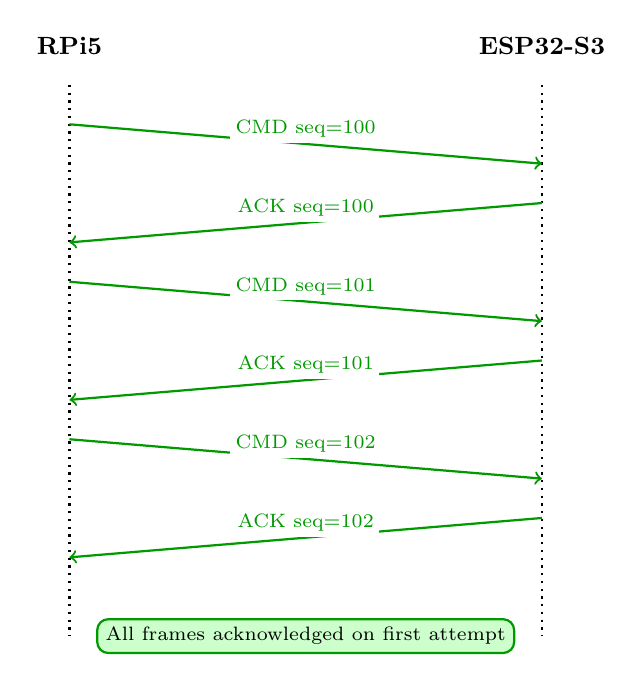
\begin{tikzpicture}[
        node distance=0.8cm,
        entity/.style={font=\small\bfseries},
        success/.style={->, thick, green!60!black},
        msgtext/.style={font=\scriptsize, fill=white, inner sep=2pt}
    ]
        % Entities
        \node[entity] (rpi) at (0, 0) {RPi5};
        \node[entity] (esp) at (6, 0) {ESP32-S3};

        % Vertical timelines
        \draw[thick, dotted] (0, -0.5) -- (0, -7.5);
        \draw[thick, dotted] (6, -0.5) -- (6, -7.5);

        % Transaction 1
        \draw[success] (0, -1) -- node[msgtext, above] {CMD seq=100} (6, -1.5);
        \draw[success] (6, -2) -- node[msgtext, above] {ACK seq=100} (0, -2.5);

        % Transaction 2
        \draw[success] (0, -3) -- node[msgtext, above] {CMD seq=101} (6, -3.5);
        \draw[success] (6, -4) -- node[msgtext, above] {ACK seq=101} (0, -4.5);

        % Transaction 3
        \draw[success] (0, -5) -- node[msgtext, above] {CMD seq=102} (6, -5.5);
        \draw[success] (6, -6) -- node[msgtext, above] {ACK seq=102} (0, -6.5);

        % Success note
        \node[font=\scriptsize, fill=green!20, draw=green!60!black, thick, rounded corners, inner sep=3pt] at (3, -7.5) {All frames acknowledged on first attempt};
    \end{tikzpicture}
    \caption{Normal ARQ Flow - Three Successful Transactions}
\end{figure}

\subsubsection{Error Recovery Scenarios}

\begin{figure}[H]
    \centering
    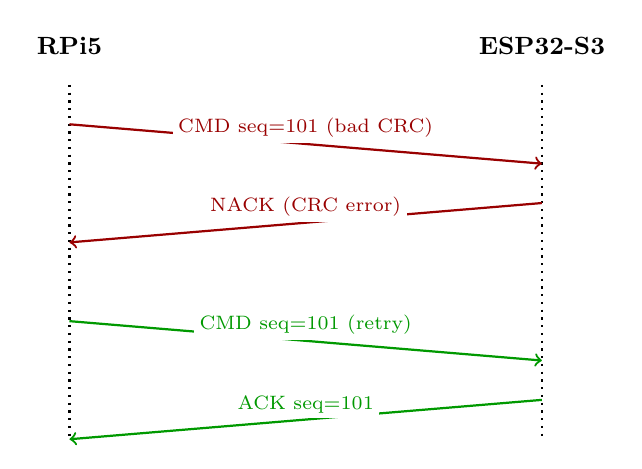
\begin{tikzpicture}[
        node distance=0.8cm,
        entity/.style={font=\small\bfseries},
        success/.style={->, thick, green!60!black},
        error/.style={->, thick, red!60!black},
        msgtext/.style={font=\scriptsize, fill=white, inner sep=2pt}
    ]
        % Entities
        \node[entity] (rpi) at (0, 0) {RPi5};
        \node[entity] (esp) at (6, 0) {ESP32-S3};

        % Vertical timelines
        \draw[thick, dotted] (0, -0.5) -- (0, -5);
        \draw[thick, dotted] (6, -0.5) -- (6, -5);

        % CRC error scenario
        \draw[error] (0, -1) -- node[msgtext, above] {CMD seq=101 (bad CRC)} (6, -1.5);
        \draw[error] (6, -2) -- node[msgtext, above] {NACK (CRC error)} (0, -2.5);
        \draw[success] (0, -3.5) -- node[msgtext, above] {CMD seq=101 (retry)} (6, -4);
        \draw[success] (6, -4.5) -- node[msgtext, above] {ACK seq=101} (0, -5);
    \end{tikzpicture}
    \caption{CRC Error - Retry with Same Sequence Number}
\end{figure}

\begin{figure}[H]
    \centering
    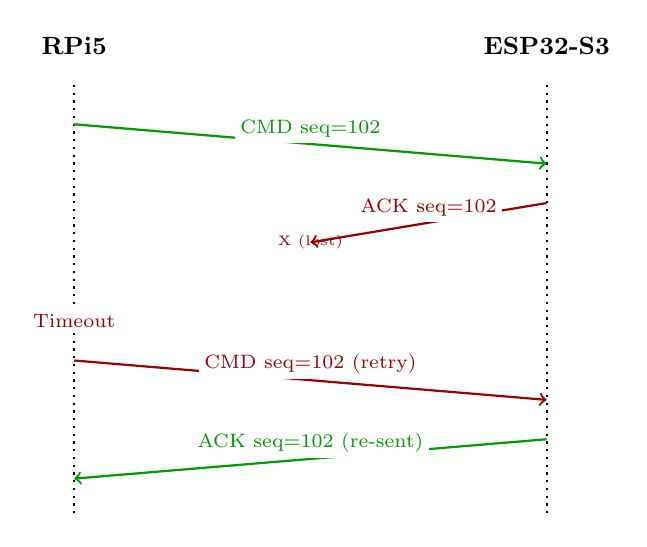
\begin{tikzpicture}[
        node distance=0.8cm,
        entity/.style={font=\small\bfseries},
        msg/.style={->, thick},
        success/.style={->, thick, green!60!black},
        error/.style={->, thick, red!60!black},
        msgtext/.style={font=\scriptsize, fill=white, inner sep=2pt}
    ]
        % Entities and timelines
        \node[entity] (rpi) at (0, 0) {RPi5};
        \node[entity] (esp) at (6, 0) {ESP32-S3};
        \draw[thick, dotted] (0, -0.5) -- (0, -6);
        \draw[thick, dotted] (6, -0.5) -- (6, -6);

        % Diagram
        \draw[success] (0, -1) -- node[msgtext, above] {CMD seq=102} (6, -1.5);
        \draw[error] (6, -2) -- node[msgtext, above] {ACK seq=102} (3, -2.5);
        \node[font=\tiny, red!60!black] at (3, -2.5) {X (lost)};
        \draw[dashed, error] (0, -3.5) -- node[msgtext] {Timeout} (0, -3.5);
        \draw[error] (0, -4) -- node[msgtext, above] {CMD seq=102 (retry)} (6, -4.5);
        \draw[success] (6, -5) -- node[msgtext, above] {ACK seq=102 (re-sent)} (0, -5.5);
    \end{tikzpicture}
    \caption{Duplicate Packet Scenario (Lost ACK)}
\end{figure}

\begin{figure}[H]
    \centering
    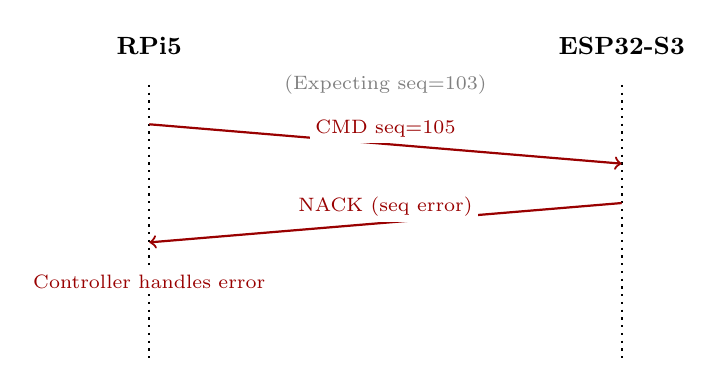
\begin{tikzpicture}[
        node distance=0.8cm,
        entity/.style={font=\small\bfseries},
        msg/.style={->, thick},
        success/.style={->, thick, green!60!black},
        error/.style={->, thick, red!60!black},
        msgtext/.style={font=\scriptsize, fill=white, inner sep=2pt}
    ]
        % Entities and timelines
        \node[entity] (rpi) at (0, 0) {RPi5};
        \node[entity] (esp) at (6, 0) {ESP32-S3};
        \draw[thick, dotted] (0, -0.5) -- (0, -4);
        \draw[thick, dotted] (6, -0.5) -- (6, -4);

        % Diagram
        \node[font=\scriptsize, gray] at (3, -0.5) {(Expecting seq=103)};
        \draw[error] (0, -1) -- node[msgtext, above] {CMD seq=105} (6, -1.5);
        \draw[error] (6, -2) -- node[msgtext, above] {NACK (seq error)} (0, -2.5);
        \draw[dashed, error] (0, -3) -- node[msgtext] {Controller handles error} (0, -3);
    \end{tikzpicture}
    \caption{Out-of-Order Packet Scenario}
\end{figure}

\begin{figure}[H]
    \centering
    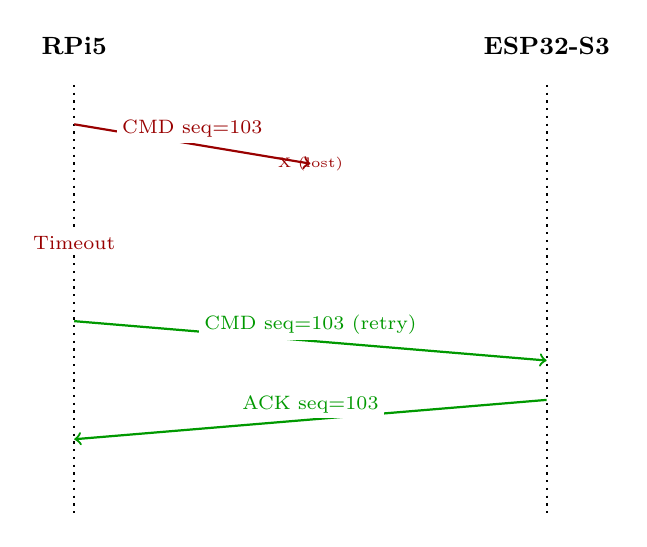
\begin{tikzpicture}[
        node distance=0.8cm,
        entity/.style={font=\small\bfseries},
        msg/.style={->, thick},
        success/.style={->, thick, green!60!black},
        error/.style={->, thick, red!60!black},
        msgtext/.style={font=\scriptsize, fill=white, inner sep=2pt}
    ]
        % Entities and timelines
        \node[entity] (rpi) at (0, 0) {RPi5};
        \node[entity] (esp) at (6, 0) {ESP32-S3};
        \draw[thick, dotted] (0, -0.5) -- (0, -6);
        \draw[thick, dotted] (6, -0.5) -- (6, -6);

        % Diagram
        \draw[error] (0, -1) -- node[msgtext, above] {CMD seq=103} (3, -1.5);
        \node[font=\tiny, red!60!black] at (3, -1.5) {X (lost)};
        \draw[dashed, error] (0, -2.5) -- node[msgtext] {Timeout} (0, -2.5);
        \draw[success] (0, -3.5) -- node[msgtext, above] {CMD seq=103 (retry)} (6, -4);
        \draw[success] (6, -4.5) -- node[msgtext, above] {ACK seq=103} (0, -5);
    \end{tikzpicture}
    \caption{Lost Packet Scenario (Timeout)}
\end{figure}


\subsection{Error Handling Strategies}

\begin{center}
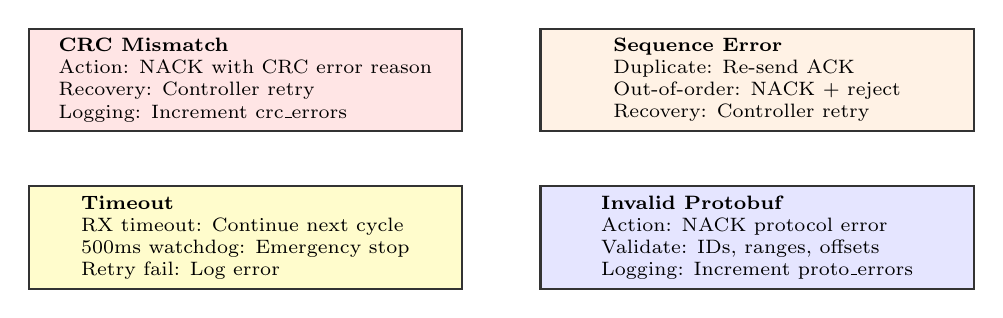
\begin{tikzpicture}[
    errorbox/.style={rectangle, draw=black!80, thick, fill=red!10, minimum width=5.5cm, minimum height=1.3cm, font=\scriptsize, align=left},
    title/.style={font=\small\bfseries}
]
    % CRC Mismatch
    \node[errorbox] (crc) at (0, 0) {
        \textbf{CRC Mismatch}\\
        Action: NACK with CRC error reason\\
        Recovery: Controller retry\\
        Logging: Increment crc\_errors
    };

    % Sequence Error
    \node[errorbox, fill=orange!10] (seq) at (6.5, 0) {
        \textbf{Sequence Error}\\
        Duplicate: Re-send ACK\\
        Out-of-order: NACK + reject\\
        Recovery: Controller retry
    };

    % Timeout
    \node[errorbox, fill=yellow!20] (timeout) at (0, -2) {
        \textbf{Timeout}\\
        RX timeout: Continue next cycle\\
        500ms watchdog: Emergency stop\\
        Retry fail: Log error
    };

    % Invalid Protobuf
    \node[errorbox, fill=blue!10] (proto) at (6.5, -2) {
        \textbf{Invalid Protobuf}\\
        Action: NACK protocol error\\
        Validate: IDs, ranges, offsets\\
        Logging: Increment proto\_errors
    };
\end{tikzpicture}
\end{center}

